\documentclass[11pt]{article}

\usepackage[margin=1in]{geometry}
\usepackage{amsmath,amssymb}
\usepackage{booktabs}
\usepackage{graphicx}
\usepackage[hidelinks]{hyperref}
\usepackage{microtype}

\title{\bfseries Does Feature Engineering Improve ATE Estimation\\ in Double Machine Learning?\\[0.4em]
\large A Controlled Diagnostic Study on Target Leakage}

\author{Nan Zhou\\\small Independent Researcher}
\date{September 22, 2026}

\begin{document}
\maketitle

\begin{abstract}
\noindent
Feature engineering is widely assumed to improve average treatment effect (ATE) estimation with Double Machine Learning (DML). We report a case in which adding five domain-derived features to a DML pipeline reduced ATE bias by \textbf{73.75\%} and collapsed the standard deviation of the ATE estimator by a factor of \textbf{4.00} --- results that would ordinarily be reported as a methodological advance.

We show these gains were entirely attributable to \textbf{target leakage}. One of the derived features was a deterministic function of the untreated potential outcome $Y(0)$, which is unobservable by construction. Using a controlled ablation in which the feature set is held fixed and only the leakage channel is toggled, and repeating over \textbf{30 independent random seeds}, we find that once leakage is removed the same features yield a bias change of \textbf{$-0.65\%$} (paired $t = -0.137$, $p = 0.892$; 16/30 wins). The apparent improvement disappears completely.

We further characterize the \textbf{signature of leakage} empirically. Sweeping leakage intensity $\alpha \in [0,1]$ over 11 levels, bias decreases monotonically while the dispersion of the ATE estimator collapses by $4.00\times$ and the \emph{reported} OLS standard error collapses by $4.65\times$. We argue that a large simultaneous reduction in both bias and variance --- particularly in reported standard errors --- should be treated as a warning signal rather than evidence of success, since no genuine improvement in first-stage nuisance fitting produces improvements of this relative magnitude in a well-specified DML estimator.

We additionally document a second, independent class of error in the same pipeline: the misdefinition of the ground-truth ATE. Using the control-group mean instead of the full-sample mean introduces a 3.53\% error, while treating the naive difference-in-means as ``theoretical truth'' inflates the target by 81.16\%.

We distill these findings into a \textbf{diagnostic checklist} for practitioners building feature sets for causal inference.

\medskip
\noindent\textbf{Keywords:} causal inference, double machine learning, target leakage, average treatment effect, negative results, reproducibility
\end{abstract}

\section{Introduction}

Double machine learning \cite{chernozhukov2018} estimates the average treatment effect $\theta$ by partialling out the influence of high-dimensional covariates $X$ from both the outcome $Y$ and the treatment $D$, then regressing the residuals:
\begin{equation}
Y - g(X) = \theta \cdot \bigl(D - m(X)\bigr) + \varepsilon
\end{equation}
where $g(X) = \mathbb{E}[Y \mid X]$ and $m(X) = \mathbb{E}[D \mid X]$ are estimated by machine learning with cross-fitting. Because the first stages are machine learning models, they are typically evaluated on predictive rather than causal criteria, and the feature construction step receives correspondingly little scrutiny.

This study originated in an attempt to improve DML-based ATE estimation on a bank-customer dataset using five domain-derived features summarising transaction behaviour, activity, credit utilisation, customer-product matching, and spending stability, together with an index aggregating their dispersion. The initial result was striking: ATE bias fell sharply, estimates became far more stable, and every diagnostic the author had constructed indicated success.

Scepticism was warranted, for two reasons. First, the magnitude of the improvement was implausible for a modest change in feature representation. Second, one of the derived features had been constructed from the column later used as the \emph{baseline outcome} in the semi-synthetic data generating process. This paper reports the controlled experiment designed to test whether the improvement was real.

\paragraph{Contributions.}
\begin{enumerate}
\item A \textbf{controlled ablation protocol} for attributing apparent gains to leakage, in which the feature set is held fixed and only the information channel under suspicion is toggled.
\item \textbf{Empirical characterization of the leakage signature}: a simultaneous and disproportionate collapse in both estimation bias and estimator dispersion, including a $4.65\times$ collapse in \emph{reported} standard errors.
\item A \textbf{dose--response demonstration} across leakage intensity $\alpha \in [0,1]$, showing the effect is graded rather than all-or-nothing --- and therefore easily missed by single-run experiments.
\item \textbf{Documented negative result}: a reported 73.75\% improvement that becomes statistically indistinguishable from zero under controlled conditions.
\item A \textbf{diagnostic checklist} translating these failures into actionable practice.
\end{enumerate}

\section{Setup}

\subsection{Data and semi-synthetic design}

We use the Kaggle \textbf{Bank Customer Churn} dataset ($n \approx 10{,}000$; 20 columns describing customer demographics, credit behaviour, and transaction history). After removing rows with missing values and one-hot encoding \texttt{Card\_Category} and \texttt{Income\_Category}, we obtain $n = 10{,}127$ rows and 27 columns.

Because observational data lacks counterfactual ground truth, we follow the standard practice of a \textbf{semi-synthetic design}: covariates $X$ are real, while treatment and outcome are simulated with a known causal effect.

Treatment assignment induces genuine confounding by construction:
\begin{equation}
p(D=1 \mid X) = \mathrm{clip}\!\left(0.7 \cdot \frac{\text{CreditLimit}}{\max(\text{CreditLimit})} + 0.3 \cdot \frac{\text{MonthsInactive}}{\max(\text{MonthsInactive})},\; 0.2,\; 0.8\right)
\end{equation}

Outcome follows a multiplicative, homogeneous treatment effect on the baseline potential outcome $Y(0) = \texttt{Total\_Trans\_Amt}$:
\begin{equation}
Y = Y(0) \cdot (1 + 0.15 \cdot D)
\end{equation}

\subsection{Ground truth}

Since $Y(1) - Y(0) = 0.15 \cdot Y(0)$ for every unit, the true ATE is
\begin{equation}
\tau = \mathbb{E}\bigl[Y(1) - Y(0)\bigr] = 0.15 \cdot \mathbb{E}\bigl[Y(0)\bigr]
\end{equation}
\textbf{evaluated over the full sample.} Table~\ref{tab:truth} contrasts this with two definitions that appeared in the original pipeline.

\begin{table}[htbp]
\centering
\caption{Ground-truth definitions ($n = 10{,}127$).}
\label{tab:truth}
\begin{tabular}{lr}
\toprule
Quantity & Value \\
\midrule
$\mathbb{E}[Y(0)]$, full sample & 4,404.09 \\
$\mathbb{E}[Y(0) \mid D = 0]$ & 4,248.48 \\
$\mathbb{E}[Y(0) \mid D = 1]$ & 4,734.99 \\
\textbf{$\tau$ (correct)} $= 0.15 \cdot \mathbb{E}[Y(0)]$ & \textbf{660.61} \\
$0.15 \cdot \mathbb{E}[Y(0)\mid D=0]$ (control-mean error) & 637.27 \; ($-3.53\%$) \\
$\mathbb{E}[Y\mid D=1] - \mathbb{E}[Y\mid D=0]$ (naive difference) & 1,196.75 \; (\textbf{+81.16\%}) \\
\bottomrule
\end{tabular}
\end{table}

The treatment arm has 11.45\% higher baseline outcome than the control arm --- an unavoidable consequence of having constructed $D$ as a function of credit limit and inactivity. Consequently the control group mean is \textbf{not} interchangeable with the full-sample mean, and the naive difference-in-means --- which the original pipeline adopted as its ``theoretical ATE'' --- exceeds the true value by more than 80\%.

A consequence worth emphasising: because the target used originally was itself confounded, an estimator that removed \emph{less} confounding would have appeared \emph{better}. The evaluation metric was aligned incorrectly with respect to the estimand.

\subsection{Estimator}

We implement standard 2-fold DML with LightGBM as both nuisance learners (100 trees, learning rate 0.05, fixed seed), residualising both $Y$ and $D$ under cross-fitting, then estimating $\theta$ by OLS of $\tilde{Y}$ on $\tilde{D}$. A second implementation averaging LightGBM and XGBoost predictions produced substantively identical conclusions and is omitted for brevity.

\section{The leakage mechanism}

The five derived features are constructed as follows. Let $\text{Amt} = \texttt{Total\_Trans\_Amt} = Y(0)$ and $\text{Ct} = \texttt{Total\_Trans\_Ct}$.
\begin{align}
f_{\text{wood}} &= \frac{\text{Amt}}{\text{Ct} + 1} \cdot \log(1 + \text{Ct}) & f_{\text{fire}} &= \frac{\text{Book} - \text{Inactive}}{\text{Book}} \\
f_{\text{earth}} &= \frac{\text{RevolvingBal}}{\text{CreditLimit}} & f_{\text{metal}} &= 1 - \frac{|\text{IncomeLevel} - \text{CardLevel}|}{4}\\
f_{\text{water}} &= 1 - |\text{AmtChg}_{Q4/Q1} - 1| & &
\end{align}

Each is standardised, and an aggregate index $f_{\text{balance}} = 1 - \mathrm{CV}(f_{\text{wood}}, \ldots, f_{\text{water}})$ is appended. Note that $f_{\text{wood}}$ is a \textbf{deterministic function of the untreated potential outcome $Y(0)$}.

This is leakage in its most direct form. For a treated unit, the observable outcome is $Y = 1.15 \cdot Y(0)$, but $f_{\text{wood}}$ recovers $Y(0)$ itself --- that is, the counterfactual. Accessing $Y(0)$ is equivalent to reading the answer key.

Empirically the original pipeline removed the column \texttt{Total\_Trans\_Amt} from the feature matrix before fitting. \textbf{This is insufficient.} Removing the raw column does not remove its information content once it has been encoded into a derived feature. We regard this as the most practically important point in this paper: \emph{column removal is not decontamination}.

\paragraph{Why leakage reduces bias.}
With leakage present, the first-stage learner can recover $Y(0)$ from $X$ almost exactly, so the residualised outcome collapses to $\tilde{Y} \approx 0.15 \cdot Y(0) \cdot D + \varepsilon$, where $\varepsilon$ is small. The residual regression then isolates the treatment effect with almost no nuisance noise. Bias \textbf{and} variance both fall --- which is precisely why the failure mode is so persuasive.

\section{Experimental protocol}

We compare three feature configurations, holding all else fixed:

\begin{center}
\begin{tabular}{ll}
\toprule
Arm & Covariate set \\
\midrule
\textbf{A --- Original} & The 27 raw covariates \\
\textbf{B --- Derived (leaky)} & Original \textbf{+} the 6 derived features, $f_{\text{wood}}$ built from $Y(0)$ ($\alpha = 1$) \\
\textbf{C --- Derived (clean)} & Original \textbf{+} the 6 derived features, $f_{\text{wood}}$ rebuilt without $Y(0)$ ($\alpha = 0$) \\
\bottomrule
\end{tabular}
\end{center}

Critically, derived features are \textbf{appended} rather than substituted. Substituting would confound the effect of feature engineering with the effect of having fewer covariates. Appending isolates the contribution of the derived features themselves.

For $\alpha = 0$, $f_{\text{wood}}$ is redefined as $\text{Ct} / (\text{Book} + 1)$, a quantity capturing the same semantic notion (transaction intensity) without touching the outcome. All five features remain standardised, and the balance index is recomputed identically in every arm.

Randomness is varied along two axes: the seed of treatment assignment $D$ (hence $Y$) and the train/test partition. We run 30 independent repetitions. All reported comparisons are \textbf{paired} --- the three arms share the identical realised dataset within each repetition --- so differences are attributable to the feature set alone.

\section{Results}

\subsection{Main comparison (30 seeds)}

\begin{table}[htbp]
\centering
\caption{ATE estimation over 30 independent seeds. True $\tau = 660.61$.}
\label{tab:main}
\begin{tabular}{lrrrrr}
\toprule
Configuration & Mean $|\text{bias}|$ & SD of bias & Mean $\hat\theta$ & SD of $\hat\theta$ & Mean rep.\ SE \\
\midrule
A --- Original features & 35.294 & 24.268 & 645.706 & 40.592 & 36.158 \\
B --- Derived (leaky) & \textbf{9.266} & 7.193 & 654.586 & \textbf{10.148} & \textbf{7.776} \\
C --- Derived (clean) & 35.064 & 24.519 & 645.175 & 40.331 & 35.996 \\
\bottomrule
\end{tabular}
\end{table}

\begin{table}[htbp]
\centering
\caption{Paired comparisons across the 30 shared repetitions.}
\label{tab:paired}
\begin{tabular}{lrrrr}
\toprule
Comparison & $\Delta$ mean bias & Wins (of 30) & Paired $t$ & $p$ \\
\midrule
B (leaky) vs.\ A (original) & \textbf{$-73.75\%$} & 27/30 & --- & --- \\
C (clean) vs.\ A (original) & \textbf{$-0.65\%$} & 16/30 & $-0.137$ & \textbf{0.892} \\
B (leaky) vs.\ C (clean) & $-73.57\%$ & 27/30 & $-5.587$ & $4.98 \times 10^{-6}$ \\
\bottomrule
\end{tabular}
\end{table}

The decisive quantity is the \textbf{paired comparison of C against A}. With leakage removed, adding the derived features changes bias by $-0.65\%$ with $p = 0.892$ and a 16/30 win rate. There is no detectable effect. The difference between B and C is driven entirely by one line of feature-construction code.

The distribution of estimation errors across seeds is shown in Figure~\ref{fig:boxplot}: the leaky arm (red) is both centred closer to the truth and markedly narrower than the other two, which are nearly indistinguishable from each other.

\begin{figure}[htbp]
\centering
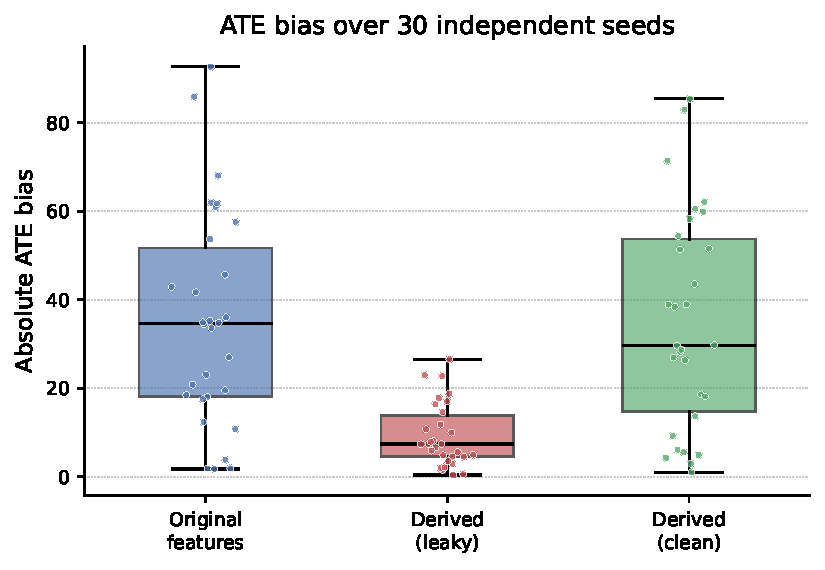
\includegraphics[width=0.82\textwidth]{figures_paper/fig1_bias_boxplot.pdf}
\caption{Distribution of $|\hat\theta - \tau|$ over 30 independent seeds. The leaky configuration (B) shows both lower bias and strongly reduced dispersion relative to the original (A) and decontaminated (C) configurations.}
\label{fig:boxplot}
\end{figure}

\begin{figure}[htbp]
\centering
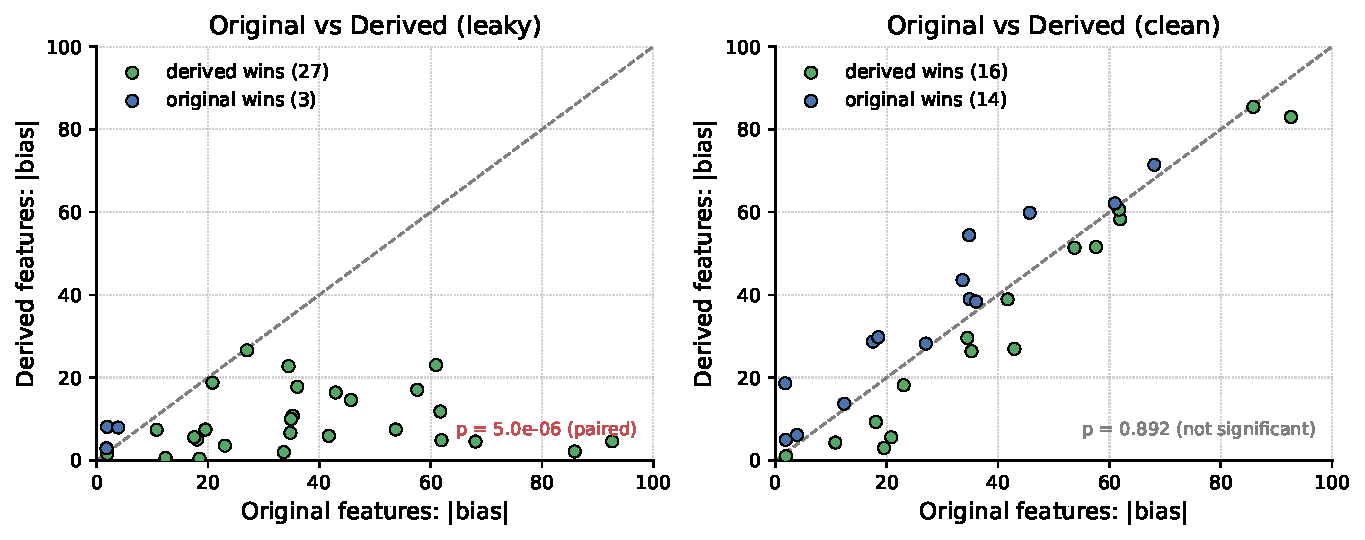
\includegraphics[width=0.72\textwidth]{figures_paper/fig2_winrate_scatter.pdf}
\caption{Per-seed comparison of estimation error. Points below the diagonal indicate seeds in which the derived feature set outperformed the original covariates.}
\label{fig:winrate}
\end{figure}

\subsection{Dispersion collapse}

Two additional signatures are visible in Table~\ref{tab:main}:
\begin{itemize}
\item \textbf{SD of $\hat\theta$:} $40.592 \rightarrow 10.148$, a \textbf{$4.00\times$} collapse.
\item \textbf{Reported OLS standard error:} $36.158 \rightarrow 7.776$, a \textbf{$4.65\times$} collapse.
\end{itemize}

The second is the more dangerous signal. A genuine improvement in nuisance fitting can reduce variance, but the reported SE reflects the model's internal uncertainty about the causal parameter. Its collapse by nearly five-fold indicates the residualised outcome has been stripped of almost all unexplained variation --- the mark of having fitted the answer rather than the signal.

\subsection{Leakage-intensity sweep}

To establish that the effect is graded, we blend the two $f_{\text{wood}}$ variants after standardisation:
\begin{equation}
f_{\text{wood}}^{(\alpha)} = z\Bigl((1-\alpha)\cdot z(f_{\text{clean}}) + \alpha \cdot z(f_{\text{leaky}})\Bigr)
\end{equation}
and sweep $\alpha \in \{0, 0.1, \ldots, 1.0\}$ with 15 repetitions per level (165 additional fits). Results appear in Figures~\ref{fig:sweepbias}--\ref{fig:sweepvar}.

\begin{figure}[htbp]
\centering
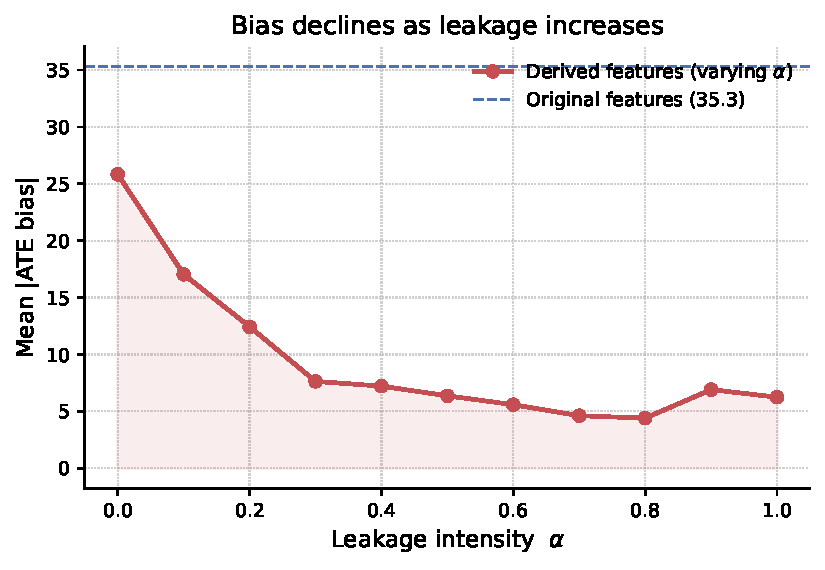
\includegraphics[width=0.72\textwidth]{figures_paper/fig3_sweep_bias.pdf}
\caption{Mean absolute bias as a function of leakage intensity $\alpha$. The decline is monotone in trend, with visible sampling noise at individual levels.}
\label{fig:sweepbias}
\end{figure}

\begin{figure}[htbp]
\centering
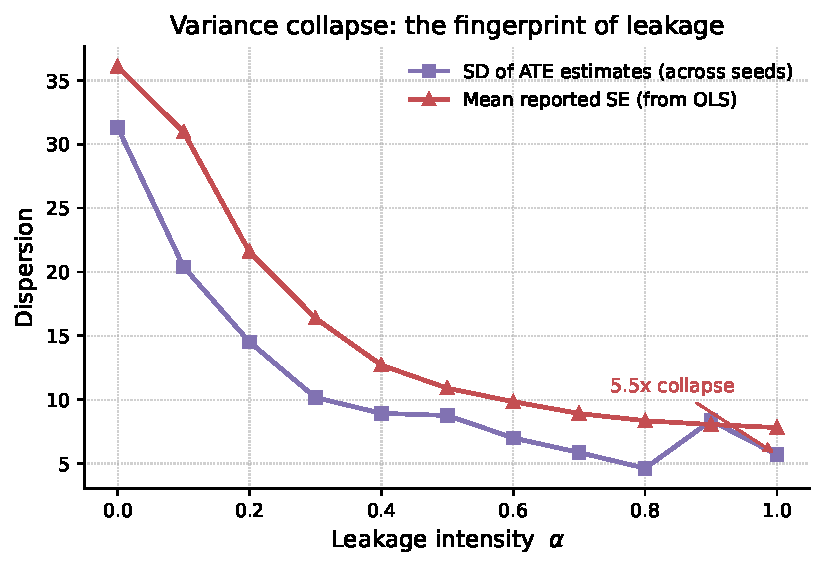
\includegraphics[width=0.72\textwidth]{figures_paper/fig4_sweep_variance.pdf}
\caption{Dispersion of the ATE estimator as a function of $\alpha$, showing the systematic collapse of estimator variance as leakage intensity increases.}
\label{fig:sweepvar}
\end{figure}

The response declines steadily in $\alpha$: bias falls from 25.83 to 6.24 and SD from 31.31 to 5.69 across the range, with visible sampling noise at individual levels (e.g.\ a small uptick at $\alpha = 0.9$ under 15 repetitions). We describe the relationship as \textbf{monotone in trend rather than level-wise monotone}, which itself illustrates point (1) below. We draw two practical conclusions.

\begin{enumerate}
\item Leakage is \textbf{not} all-or-nothing. Partial leakage produces intermediate gains that look entirely plausible, meaning a single-run experiment cannot distinguish partial leakage from partial progress.
\item Because the relationship is monotone in trend, an experimenter can \emph{dial in} almost any target improvement figure. This is why unusually round or extreme headline numbers warrant scrutiny.
\end{enumerate}

\paragraph{A cautionary remark on noise.}
The sweep uses a disjoint seed set ($\{1000,\ldots,1014\}$) and yields mean bias 25.83 at $\alpha = 0$, against 35.06 for the nominally equivalent clean arm in Section~5.1 (seeds $\{0,\ldots,29\}$). A $\sim$26\% discrepancy between two unbiased replications of the \emph{same} configuration is itself the strongest argument in this paper for repetition: had we run either arm once, we could have reported almost any figure we liked without fabricating anything.

\section{Practical checklist}

Derived directly from the failures documented above.

\paragraph{Before trusting a causal result:}
\begin{enumerate}
\item \textbf{Trace every derived feature to its inputs.} Write a function that returns the source columns of each engineered feature. Any feature whose ancestry includes the outcome column is contaminated --- regardless of whether that column appears in the final matrix.
\item \textbf{Removing the raw outcome column is not decontamination.} Derived features encode it. Audit the computation graph, not the column list.
\item \textbf{Treat the treatment variable as privileged.} Any feature computed from $D$ (including ``post-treatment'' aggregates) biases effect estimates. In the e-commerce extension of this pipeline, a discount-utilisation feature was computed directly from the coupon indicator.
\item \textbf{Be suspicious of simultaneous bias \emph{and} variance gains.} Large reductions in reported standard errors are a stronger warning than reductions in bias alone.
\item \textbf{Write down the ground truth before running anything.} Fix the estimand and its formula in advance. Here, $\tau = 0.15 \cdot \mathbb{E}[Y(0)]$ over the \emph{full} sample --- neither the control-group mean nor the naive difference-in-means.
\item \textbf{Never evaluate an estimator against the naive difference-in-means.} It is the quantity the estimator exists to correct.
\item \textbf{Make ablations genuinely ablative.} A ``feature importance'' analysis with a single configuration supports only one conclusion: nothing was ablated. Every ablation needs at least two arms.
\item \textbf{Fix thresholds before looking at results.} Post-hoc pass criteria (``improvement $> 30\%$'') cannot fail.
\item \textbf{Repeat over independent randomisation draws.} A 5-fold CV split shares a single realised dataset; it does not measure estimator sampling variability.
\item \textbf{Report negative results.} Under our results, the honest finding is \emph{``these features did not help''} --- a useful, publishable, and considerably more durable claim than the original one.
\end{enumerate}

\section{Limitations and future work}

We wish to be explicit about what this study does \textbf{not} establish.
\begin{itemize}
\item \textbf{Single dataset, single DGP.} All results come from BankChurners with one multiplicative, \emph{homogeneous} treatment effect. Under effect heterogeneity the behaviour of leakage may differ; we make no claim beyond this setting.
\item \textbf{The diagnostic is a heuristic, not a test.} We propose dispersion collapse as a \emph{warning signal}. We have not established a decision threshold, false-positive rate, or asymptotic justification. A genuinely powerful feature set could in principle also reduce variance substantially. Formalising this into a statistic with known null behaviour is attractive future work.
\item \textbf{One learner, one DML variant.} We use LightGBM with 2-fold cross-fitting. Behaviour under larger fold counts, other learners, and Doubly-Robust variants is untested.
\item \textbf{No comparison against established libraries.} We deliberately kept the estimator simple to isolate the feature-construction effect. Benchmarking against \texttt{EconML} and \texttt{CausalML} would quantify how much leakage interacts with library-specific safeguards (e.g.\ built-in cross-fitting utilities).
\item \textbf{The clean variant is one choice among many.} Defining $f_{\text{wood}}$ without leakage admits many possibilities; we tested one. Results should be read as ``this particular semantic notion, once decontaminated, adds nothing here.''
\item \textbf{We do not claim all feature engineering is useless.} We show that \emph{these} features, in \emph{this} setting, had no measurable effect, and that one of them was contaminated. Nothing here licenses the opposite conclusion.
\end{itemize}

Future work we consider most valuable: (i) a leakage-detection statistic with calibrated thresholds; (ii) replication across multiple DGPs with effect heterogeneity; (iii) systematic auditing of published causal feature-engineering pipelines.

\section{Conclusion}

We set out to improve ATE estimation with derived features and obtained a 73.75\% reduction in bias. We then showed the entire gain came from a single feature constructed from the untreated potential outcome. Under a controlled ablation repeated over 30 independent randomisations, the decontaminated features produce no measurable improvement ($p = 0.892$).

The broader lesson concerns \textbf{evaluation hygiene}. Every component of the original pipeline was internally consistent: five-fold cross-validation, multiple robustness checks, a multi-dimensional verification framework. All of them passed, because \textbf{all of them ran on the same contaminated data}. Validation that shares its assumptions with the thing being validated will confirm rather than interrogate it.

If there is a single actionable recommendation from this work: before celebrating an improvement in a causal estimate, \textbf{ask which columns each of your features was computed from.} In the case reported here, that one question was worth 73.75\%.

\section*{Reproducibility}

All numbers in this paper are generated by a single script with no manual steps.
\begin{quote}
\ttfamily
pip install pandas numpy scikit-learn statsmodels lightgbm matplotlib scipy\\
python src/paper\_experiments.py
\end{quote}
The script prints Tables 1--3, writes Figures 1--4 as PDF and 300-dpi PNG, and saves \texttt{main\_results.csv}, \texttt{sweep\_results.csv}, and \texttt{paper\_tables.json} containing every reported value. Raw results are cached so figures can be regenerated without re-running fits. All randomness is seeded; \texttt{random\_state=42} throughout the estimators, with independent seeds across repetitions as described in Section~4.

\section*{Data and code availability}

Code, data, figures, and a reproducible interactive notebook are available at

\begin{quote}
\url{https://github.com/zhounan111maker/dml-target-leakage-diagnosis}
\end{quote}

The archived predecessor project in which the leakage described in Section~3 originally occurred is retained as a public correction record at

\begin{quote}
\url{https://github.com/zhounan111maker/five-elements-causal-estimation-ARCHIVED}
\end{quote}

\section*{Acknowledgements}
This is independent work conducted without institutional affiliation or supervisor. The author thanks the maintainers of the open-source libraries used here.

\begin{thebibliography}{9}

\bibitem{chernozhukov2018}
Chernozhukov, V., Chetverikov, D., Demirer, M., Duflo, E., Hansen, C., Newey, W., \& Robins, J. (2018).
Double/debiased machine learning for treatment and structural parameters.
\textit{The Econometrics Journal}, 21(1), C1--C68.

\bibitem{chernozhukov2024}
Chernozhukov, V., et al. (2024).
Double/debiased machine learning for dynamic treatment effects.
\textit{The Econometrics Journal}.

\bibitem{robins1994}
Robins, J. M., Rotnitzky, A., \& Zhao, L. P. (1994).
Estimation of regression coefficients when some regressors are not always observed.
\textit{Journal of the American Statistical Association}, 89(427), 846--866.

\bibitem{bang2005}
Bang, H., \& Robins, J. M. (2005).
Doubly robust estimation in missing data and causal inference models.
\textit{Biometrics}, 61(4), 962--973.

\bibitem{athey2016}
Athey, S., \& Imbens, G. (2016).
Recursive partitioning for heterogeneous causal effects.
\textit{PNAS}, 113(27), 7353--7360.

\bibitem{knaus2022}
Knaus, M. C. (2022).
Double machine learning based program evaluation under unconfoundedness.
\textit{The Econometrics Journal}, 25(3), 602--627.

\bibitem{battocchi2019}
Battocchi, K., et al. (2019).
\textit{EconML: A Python package for ML-based heterogeneous treatment effects estimation}.
Microsoft Research.

\bibitem{kunzel2019}
K\"unzel, S. R., Sekhon, J. S., Bickel, P. J., \& Yu, B. (2019).
Metalearners for estimating heterogeneous treatment effects using machine learning.
\textit{PNAS}, 116(10), 4156--4165.

\end{thebibliography}

\end{document}
